\documentclass[a4paper,11pt]{article}
\usepackage[utf8]{inputenc}
\usepackage[english]{babel}
\usepackage{url} %url parsing
\usepackage[colorlinks, allcolors=blue]{hyperref} %advanced referencing options
\usepackage{float} %better images/tables positioning
\usepackage{graphicx} %better image insertion
\usepackage{amsmath} %text in equasions (include the 2 packages below)
\usepackage{amsfonts}
\usepackage{amssymb}
\usepackage{IEEEtrantools}
\usepackage{outlines} %sub-items in lists
\usepackage{fancyhdr}
\usepackage{csquotes} %more consistent quotes
\usepackage{comment}
\usepackage[backend=bibtex,bibencoding=utf8]{biblatex}
\usepackage[parfill]{parskip} %Sane paragraphs at last! The same can be acheived with the 2 lines below:
%\setlength{\parskip}{5pt}
%\setlength{\parindent}{0pt}
\usepackage{neuralnetwork}
\usepackage{caption}
\usepackage{xcolor}
\usepackage{listings}
\usepackage{titlesec}
\setcounter{secnumdepth}{4}
\setcounter{tocdepth}{4}
\titleformat{\paragraph}
{\normalfont\normalsize\bfseries}{\theparagraph}{1em}{}
\titlespacing*{\paragraph}
{0pt}{3.25ex plus 1ex minus .2ex}{1.5ex plus .2ex}
\usepackage{tikz}
\usetikzlibrary{automata,positioning,shapes.geometric,fit}
\bibliography{mybib.bib}
\pagestyle{fancy}
\extramarks{\markboth}{}
\lhead{\markboth}
\rhead{\thepage}
\begin{document}
\pagenumbering{gobble}
\thispagestyle{empty}
\title{Exploring the impact of language differences on GANs for password cracking}
\author{Eugeio Maria Capuani}
\maketitle
\cleardoublepage
\pagenumbering{arabic}
%  A simple AAU report template.
%  2015-05-08 v. 1.2.0
%  Copyright 2010-2015 by Jesper Kjær Nielsen <jkn@es.aau.dk>
%
%  This is free software: you can redistribute it and/or modify
%  it under the terms of the GNU General Public License as published by
%  the Free Software Foundation, either version 3 of the License, or
%  (at your option) any later version.
%
%  This is distributed in the hope that it will be useful,
%  but WITHOUT ANY WARRANTY; without even the implied warranty of
%  MERCHANTABILITY or FITNESS FOR A PARTICULAR PURPOSE.  See the
%  GNU General Public License for more details.
%
%  You can find the GNU General Public License at <http://www.gnu.org/licenses/>.
%
%
%
% see, e.g., http://en.wikibooks.org/wiki/LaTeX/Customizing_LaTeX#New_commands
% for more information on how to create macros

\newcommand{\nl}{ \\[1\baselineskip]}

%1 width, 2 path, 3 caption
%How to use: \picit{0.8}{figures/certificate.png}{A caption}{A label}
\newcommand{\picit}[4]{
	\begin{figure}[H]
    	\captionsetup{width=0.5\linewidth}
 		\centering
    	\includegraphics[width=#1\textwidth]{#2}
  		\caption{#3}
        \label{#4}
	\end{figure}
    %\noindent
}

%%%%%%%%%%%%%%%%%%%%%%%%%%%%%%%%%%%%%%%%%%%%%%%%
% Macros for the titlepage
%%%%%%%%%%%%%%%%%%%%%%%%%%%%%%%%%%%%%%%%%%%%%%%%
%Creates the aau titlepage
\newcommand{\aautitlepage}[3]{%
  {
    %set up various length
    \ifx\titlepageleftcolumnwidth\undefined
      \newlength{\titlepageleftcolumnwidth}
      \newlength{\titlepagerightcolumnwidth}
    \fi
    \setlength{\titlepageleftcolumnwidth}{0.5\textwidth-\tabcolsep}
    \setlength{\titlepagerightcolumnwidth}{\textwidth-2\tabcolsep-\titlepageleftcolumnwidth}
    %create title page
    \thispagestyle{empty}
    \noindent%
    \begin{tabular}{@{}ll@{}}
      \parbox{\titlepageleftcolumnwidth}{
        \iflanguage{danish}{%
          
\includegraphics[width=\titlepageleftcolumnwidth]{figures/ruc}
        }{%
          
\includegraphics[width=\titlepageleftcolumnwidth]{figures/ruc}
        }
      } &
      \parbox{\titlepagerightcolumnwidth}{\raggedleft\sf\small
        #2
      }\bigskip\\
       #1 &
      \parbox[t]{\titlepagerightcolumnwidth}{%
      \textbf{Abstract:}\bigskip\par
        \fbox{\parbox{\titlepagerightcolumnwidth-2\fboxsep-2\fboxrule}{%
          #3
        }}
      }\\
    \end{tabular}
    \vfill
    \iflanguage{danish}{%
      \noindent{\footnotesize\emph{Rapportens indhold er frit tilgængeligt, men offentliggørelse (med kildeangivelse) må kun ske efter aftale med forfatterne.}}
    }{%
      \noindent{\footnotesize\emph{
      %The content of this document is freely available, but publication (with reference) may only be pursued due to agreement with the author.
      }}
    }
    \clearpage
  }
}

%Create english project info
\newcommand{\englishprojectinfo}[8]{%
  \parbox[t]{\titlepageleftcolumnwidth}{
    \textbf{Title:}\\ #1\bigskip\par
    %\textbf{Theme:}\\ #2\bigskip\par
    \textbf{Project Period:}\\ #3\bigskip\par
    \textbf{Project Group:}\\ #4\bigskip\par
    \textbf{Participant(s):}\\ #5\bigskip\par
    %\textbf{Supervisor(s):}\\ #6\bigskip\par
    %\textbf{Copies:} #7\bigskip\par
    \textbf{Page Numbers:} \pageref{ch:initial_design_doc}\bigskip\par
    \textbf{Date of Completion:}\\ #8
  }
}

%Create danish project info
\newcommand{\danishprojectinfo}[8]{%
  \parbox[t]{\titlepageleftcolumnwidth}{
    \textbf{Titel:}\\ #1\bigskip\par
    \textbf{Tema:}\\ #2\bigskip\par
    \textbf{Projektperiode:}\\ #3\bigskip\par
    \textbf{Projektgruppe:}\\ #4\bigskip\par
    \textbf{Deltager(e):}\\ #5\bigskip\par
    \textbf{Vejleder(e):}\\ #6\bigskip\par
    \textbf{Oplagstal:} #7\bigskip\par
    \textbf{Sidetal:} \pageref{LastPage}\bigskip\par
    \textbf{Afleveringsdato:}\\ #8
  }
}

\thispagestyle{empty}
\begin{abstract}
The goal of this thesis is to explore what impact language has on password cracking (if any) when using Generative Adversarial Networks (GANs) to crack passwords.
In it we build on existing research by taking an existing GAN-based password cracker, and testing it with a dataset of leaked user passwords from Italy. 
By comparing the performance of the resulting model with widely-used wordlists based primarily on English-language sources, as well as state-of-the-art rule-based tools, we hope to get insights into the impact that different grammatical structures have on both the performance of the GAN model, and by extension on its performance as a password cracking tool.

To that end we also wish to explore whether including Italian language corpora during training is decremental to the network's performance (as some prior research seems to indicate), or if it can prove beneficial in this particular context. 
\end{abstract}

\cleardoublepage
\section{Introduction}\label{sec:introduction}
\subsection{Motivation}
The aim of this thesis is to evaluate the paper \enquote{PassGAN: A Deep Learning Approach for Password Guessing}\cite{PassGAN}, by testing the Deep Learning system described in the paper with a different dataset of leaked passwords from Italy\cite{libero_leak} (referred to as the Libero dataset in this paper). Te aim is to test whether there are any differences in performance when PassGAN is used to crack a database from a non-english source.

This dataset is composed of real user passwords belonging to the Italian email provider Libero Mail, that were leaked in 2016. %We believe the use of these passwords to be ethical because this particular leak has been public for a number of years. %And the company has since taken action to remediate?

The underlying tough behind this it to test whether differences in grammar and language have any noticeable effect when training the system: perhaps GANs are expressive enough that they 
can account for the different provenance of the data without any significant change, or maybe some adjustments should be made such as the inclusion of Natural Language corpora on the training data. Another possible change might be to mix password datasets from English and non-English sources.

The inclusion Natural language corpora might present its own challenges, such as the fact that some prior studies with GANs and RNNs indicates that the inclusion of such data ends up creating a lot of noise rather than improving performance\cite{Melicher2016}.

One might make the case that linguistic differences are not that relevant when it comes to passwords, that the use of grammatical constructs is often trumped by patters of user behaviour in password creation that are international and well represented in rule-based password crackers. Thus, it should not matter where the network learns these patterns.\\
On the other hand, in our early attempts to train PassGAN on the Libero dataset we observed that most of the passwords the system generates attempt to mimic the sound and structure of Italian words; This leads us to speculate that the inclusion on natural language corpora might help the system to generate grammatically correct words, and thus perhaps improve performance.

In conclusion, we believe this research might contribute some insight in the role that grammatical features have in password cracking, when this task is approached using Deep Neural Networks: many papers on the subject (including \cite{PassGAN} and \cite{Melicher2016}) ask the question of whether Deep Learning systems are expressive enough to generate novel passwords and thus yield results that are not achievable with traditional password cracking methods, and we see this research as part of this ongoing quest into exploring the capabilities and limits of Deep Learning-based password crackers.

\subsection{Problem formulation}\label{subsec:problem-formulation}
This Thesis aims to answer the following questions:
\begin{itemize}
\item How does PassGAN perform when cracking italian passwords? %Implies: is it better or worse when using the pre-trained model as opposed to a new model trained on italian passwords?
\item Does difference in language have an impact on the passwords found by PassGAN and state-of-the-art password crackers?    
\item How does the inclusion of natural language data during training affect PassGAN's performance?
\item Ultimately, can PassGAN be a useful tool to use when approaching password data from a particular language area? %Or are rule-based tools always better    
\end{itemize}


\cleardoublepage
%THE ONLY CHANGE LEFT TO IMPLEMENT IS THE DIAGRAM DEPICTING WORDLISTS AND RULES.
%REMEMBER TO SPELL-CHECK THIS SECTION AGAIN

%The main process of encoding is hashing not encryption! doont mention encryption if you can.
%encryption is a 2 way fnction cuz you can decrypt andd encypt, there s no decrypt fr hashes.
\section{Related Work}\label{sec:related_work}
Both Password Cracking and Deep Learning are active areas of research developing at a rapid pace.

In section 2, we aim to give an overview of the relevant knowledge in these areas as it relates to our thesis: section \ref{subsec:password_cracking} below will cover the relevant knowledge concerning passwords, while section \ref{subsec:deep-learning} will cover Deep Learning.

\subsection{Password Cracking}\label{subsec:password_cracking}
Password cracking has been around for a long time, and while technology has evolved greatly and continues to do so, the basic concepts have remained relatively similar:
back in 1979, Morris and Thompson were already aware of different ways to attack passwords and defend against such attacks \cite{Thompson1979}.

At the base of all password attacks is the concept of \emph{key space}, i.e the set of all possible passwords of a certain length that use a specific character set \cite{Thompson1979,hash_cat_mask_attack}. 

Key space can be formally defined as the set of all possible keys for some given parameters. The two parameters in question are: the Alphabet of the key (the set of all symbols or characters used in the key), and the length of the key.
Key space can be theoretically infinite, but in practice it is bound by both the alphabet and the key length: in the case of an hexadecimal key of length 10, the key space can be quantified as $16^{10}$ possibilities; on the other hand in the case of the password \texttt{password} (written with lowercase characters only), the key space can be expressed as $26^8$. %convert keyspace sizes to power of 2 to compare the size in bits

Key space is important because it forms the basis from which password cracking techniques work off: if the password is sufficiently complex, an attacker will have to do an exhaustive search of the key space in order to find the password. 
It follows then, that one of principles of password strength is to make the search space big enough to be impractical to search through with current hardware.
This is the reason why users are commonly advised to use a variety of different characters classes in their passwords, and also to use passwords of a certain minimum length.

To ground our discussion of search space in the context of cracking, we should address how passwords are stored in the first place: As Morris and Thompson explain in their paper, the simplest approach is to store the users' passwords in a file or database as they are entered: this is a bad idea as any software bug that causes an accidental disclosure will leave the users exposed, and also because any privileged user can simply look up other users' passwords.

A better approach would be to somehow encrypt the user's password, and store the cypher text: when a user logs in, the string they typed is encrypted, compared with the cypher text and access is granted if it matches. This process is commonly achieved through a one-way cryptographic hash function, while Morris and Thompson use the DES algorithm in their paper.

%DES is an encryotion algo but they used it for hasing. also the proper name for a hash is "cryptographic hash function"
Simply put, a cryptographic hash function is a mathematical function that encodes a string in a predictable way, mapping an arbitrary amount of input (a message of arbitrary length) to a string of a fixed length (a hash). 

Cryptographic hash functions adhere to strict security standards (hence the adjective \enquote{cryptographic}) but they different from encryption algorithms like AES or GPG:
one of the main differences between encryption and hashing algorithms is that an hashing algorithm is a one-way function, meaning there is no mechanism to decrypt or otherwise reverse the process once the input data has been hashed. 

Another difference can be found in the purpose of hashing algorithms: broadly speaking they are used to compress information about an arbitrary amount of data into a string of a certain length; their main application is to act as \enquote{fingerprints} for a given message, ensuring the integrity and/or authenticity of the data rather than its confidentiality.

The reason why they are used with passwords is that in a scenario like the one mentioned above (where whatever string the user types is hashed and compared with the hash in the database) there is no need for decryption: yes the hash algorithm obscured the input, but its main role its to make sure the password the user enters at login is the same as the one that is stored in the database.
Additionally, the mere possibility of decrypting a user's password might represent a security risk: if a user forgets a password we do not need to  decrypt it and show it to the user, we can simply delete the password and ask him to make a new one. 

Crucially, in order to accomplish its task a hashing algorithm needs to be predictable i.e always output the same string for a given input: this is a propriety an attacker can exploit as we will see shortly. 

When a strong hashing algorithm is used, an attacker will theoretically have to do a key space search in order to crack the users' password: this process will take even more time, as every candidate string/password must be first hashed with the same algorithm and then looked up in the database.

Hashing alone does not solve the problem however, because in reality an attacker would not have to resort to brute-forcing in a majority of cases.

Because the hashing algorithm needs to always output the same result for a given input string, the attacker can start comparing the hashes in the database and draw some conclusion: if some hashes appear many times, they probably hold the plain text of some very common passwords; if the attacker cracks those first and starts looking for similar patterns, he may crack a sizable number of the passwords contained in the database.

Practically, an attacker can exploit this predictability by building a table with pre-computed hashes for all the most common passwords: this technique saves a lot of time since we do not need to encrypt every candidate password before comparing it with the database, and instead we merely look up the hashes from the table in the database. 

These tables are commonly referred to as \emph{Rainbow Tables}, and they are a simplified version of the rule-based techniques covered in section \ref{hash_and_jtr}.

Rainbow tables can be defeated by using \emph{password salting}: salting works by generating a random string that is then appended to the user's password before it is hashed (mainly when the user first creates the account). The authors in \cite{Thompson1979} use a 12-bit random number as their salt, but modern sources suggest the use of longer and more complex salts \cite{NIST_2017}; by generating a unique salt per each user (or even better, per each individual password a user creates), rainbow tables and correlation attacks will be rendered useless as its no longer possible to generate hashes of passwords that will work on the target; one might attempt to generate tables that contain salts, but this is impractical as it would mean brute-forcing the key space of the salt.
This can be done however in cases where the salt is very short, or alternatively when the system administrators have chosen one fixed salt string with which every password is processed.
The latter mistake its particularly grave, as it defeats the purpose of having salts in the first place.
   
% Let us suppose that an attacker has access to both the hashed passwords of the users and the salts that each password uses: it is conceivable that one might extract all the salts from the database, put them in a dictionary, and use them in a rule-based dictionary attack such as the ones that will be described in section \ref{hash_and_jtr}: if the salt for each user is stored in the database, we do not need to brute-force the key space of the salt: every salt belongs to one of the users, hence we merely need to try them all sequentially on every password candidate. 
% A remedy for such scenario is offered in \cite{NIST_2017} and will be discussed further down. %FUCK ME WITH A RUSTY SPEAR, I HAVE NO IDEA IF THIS IS BS I JUST MADE UP!

For a more current example of how these security practices have evolved since 1979, we can look at the National Institute of Standards and Technologies' standard SP 800-63-3.
This standard is intended to provide security guidelines for information systems within the US government, and was released in June 2017.

Document SP 800-63-3B \cite{NIST_2017}, provides guidelines on how user secrets (passwords and/or PINs) should be stored.\\
They suggest that user passwords should be between 8 and 64 characters, but advise against enforcing password policies concerning the composition of passwords; Instead, they suggest that user passwords be checked against a list of leaked passwords and dictionary words before they are accepted, in order to avoid the use of weak passwords.

When it comes to encryption, they suggest the use of the PBKDF2 and Balloon algorithms; Other hashing algorithms listed as suitable for password encryption include HMAC and SHA-3.

Furthermore, they recommend that all passwords be salted with at least a 32bit quantity; to our understanding the standard calls for a unique salt for each user, as opposed to a unique salt for each password. The salts should be stored alongside the hashed password of the user.

In order to foil dictionary attacks in cases where the attacker has access to the users' salts alongside the hashes, the system should perform an additional iteration of the encryption algorithm using a different 112bits salt that should be secret and stored on separate hardware form the main database.\\
If we were to apply such process before encrypting the users password with the standard 32bit salt, this would effectively neutralize all dictionary attacks even when the attacker factors the salts into the process.

To conclude this discussion of password storage and security, we will briefly touch upon our main dataset used in the thesis: the Libero dataset.

The Libero dataset is a JSON formatted document that contains information on roughly 700 thousand users of the italian email provider Libero Mail \cite{libero_leak}.\\
Each user record contains various fields such as  user ID, user name, the associated email address and the user's password in plain text.
These plain text passwords served as the basis for all our experiments (detailed in section \ref{sec:testing_and_evaluation}), in which we attempted to crack the Libero dataset with rule-based password crackers and PassGAN. Because the passwords were provided in plain text, we had to hash them with MD5 in order to crack them.
The fact that our dataset did not contain hashed passwords presented a problem, and called into question the authenticity of the data in our possession: we will go into further detail with this  and the choices we made regarding the cracking process in section \ref{sec:libero}.  

Now that we have a better notion of how passwords are stored, the next section will address how passwords are commonly cracked: specifically, we will use state of the art rule-based password crackers in order to explore the cracking process. % to briefly elucidate on how these tools fit in the greater scope of the paper, PassGAN and other such Deep Learning systems can be seen as a complement to rule-based password crackers, as their output is used as input for rule-based tools in order to practically crack passwords. The interplay between these two sides will be explored in section \ref{sec:testing_and_evaluation}.


%Add a diagram with the process of applying rules and using wordlists
\subsubsection{Rule-Based password crackers} \label{hash_and_jtr}
Unlike other password cracking tools made for brute-forcing passwords, rule-based tools rely on their name sake in order to attack a greater variety of passwords:

Mangling rules are patters that define how a string should be modified, they can be given in either in a regular language or in a more complex form.
Their purpose is to modify each string in a wordlist or dictionary so that one entry in the wordlist can match multiple, similar passwords.\\

The simplest kind of rules are \emph{masks}: they are a subset of mangling rules whose use will be explained in section \ref{par:brute-force}. Masks are patterns expressed in a regular language, that define what character classes are in a password and at what position: their main function is to shrink the key space when executing brute-force attacks.

\enquote{Proper} mangling rules by contrast are more complex and more expressive, in line with a context-free or context-sensitive language; they will be covered is section \ref{par:rule-based}.
Common examples of rules might be a rule that switches the case of the first letter of the string (mainly in order to capitalize passwords, a common strategy users employ to comply with password composition requirements), or a rule that appends one or two digits to the end of a string. 

Two common rule-based password cracking tools are John The Ripper and \break \mbox{HashCat}\cite{john,hash_cat}: these tools use rules to exploit common patterns in user behaviour in order to optimize the cracking process: Both tools have a variety of techniques an attacker can employ, and we will briefly exemplify their capabilities using HashCat as an example \cite{hash_cat_wiki}:

In both tools there are three categories of attacks that can be carried out: brute-force attacks, dictionaries attacks and rule-based attacks: these can be combined and tweaked in various ways depending on the desired result, and there is a degree of overlap between each.


\begin{itemize}
\item Brute-force attacks try every possible combination of characters within a defined pattern, and thus closely relate to keyspace search. 
\item Dictionary attacks use a dictionary of words or passwords as a source for password candidates, that are hashed and checked against the target to see if any of them match
\item Rule-based attacks are an evolution of Dictionary attacks, in which the dictionary's effectiveness is boosted by some mangling rules that change the words in ways that reflect common patterns in user-generated passwords.
\end{itemize}

HashCat distinguishes between brute-force attacks and wordlist-based attacks with two separate modes (a mode is a setting that defines the kind of attack that HashCat should carry out), but there is no such distinction between wordlist-based attacks and Rule-based attacks: instead rules are an optional parameter one can use in wordlist attack mode to greatly increase the effectiveness of the wordlist. The following three sections will cover HashCat's attack strategies by the different modes present in the software. 

\paragraph{Brute-force attacks}\label{par:brute-force}
The simplest of these modes is \emph{Mask attack} mode, used to carry out brute-force attacks as we mentioned previously: a mask attack is essentially an optimized version of key space search, meant to attack simpler passwords while shrinking the key space search. 
Instead of searching the total space for a password of length $x$, we define a simple regular pattern expressing the what character classes are there and at which position, saving us a substantial amount of processing time.
For example if we have a password like \texttt{Benjamin86} or \texttt{Iloveyou02}, we can capture both examples by defining a pattern to be a ten-character string with eight lowercase or uppercase letters and two numbers at the end; This is referred to as a \emph{Mask} in HashCat's documentation:

In a classic brute-force attack we would deal with a search space of $62^{10}$ (or roughly $8 \times 10^{17}$ combinations), but thanks to the above-mentioned mask we can reduce our search space to around $4 \times 10^{13}$ possibilities if we assume that the first character in the string is the only one that can be uppercase.
Furthermore we can use the \texttt{--increment } option in HashCat to apply this mask recursively, to all strings up to ten characters: this allows us to match shorter passwords that follow the same pattern.

This method is rather simplistic and not very flexible, but exemplifies some of the ways in which attackers can optimize key space attacks.

\paragraph{Dictionary attacks}
The main mode of operation oh HashCat \emph{straight} mode, that performs a dictionary attack: In this mode, the program is fed a wordlist/dictionary, and tries each entry the wordlist as a password candidate. Because of its simplicity, such a dictionary attack works best with a wordlist composed of leaked passwords; the aim is to target very common passwords and users that re-use passwords, but the effectiveness of such an attack can increase significantly depending on what wordlist is used.

Dictionary attacks can be further enhanced by combining them in various ways: one approach would be to use two wordlists and append/prepend each entry in the second one to each entry in the first.\\ 
The second wordlist might be a natural language dictionary or simply anther wordlist of plain-text leaked passwords. This is called \emph{Combinator attack} mode in HashCat. 

We might also want to use the output of a mask attack as our second wordlist: If we use the patterns described in the Mask Attack mode to generate strings or number sequences we combine with a wordlist, we will obtain a more targeted and effective version of the Mask Attack method. 

For example if we know that a good deal of the passwords we want to extract are strings with numbers appended to the end, we might run a mask that generates combinations of 0 to 4 digits and then combine the output of that with our wordlist. This is called \emph{Hybrid attack} mode in HashCat.

\paragraph{Rule-based attacks}\label{par:rule-based}
Finally we come to rule-based attacks, In short they are an extension of all the methods described above. 
As we said previously  rule-based attacks do not have a dedicated mode, but instead they are often used in \emph{straight} mode alongside a wordlist in order to boost the number of passwords found by that wordlist.

Rules are flexible and allow for more thorough definition of the patterns that may appear in a password, going beyond the capabilities of the regular language used with Masks.
Patterns can be created independently of the size and characteristics of the passwords, and they are not limited to a fixed patterns; there are also flow control statements and options to apply rules only in certain conditions.
There are also options to save password candidates to memory enabling more advanced processing: saved strings can be appended to each password candidate matching certain criteria, reversed and so on...
These more advanced options allow an attacker to emulate the operation of both Combinator and Hybrid attacks using just mangling rules. 

Rules are applied once to each entry in a wordlist in a similar way to a combinator attack, but multiple rules can also be be applied sequentially to a memorized password or string.

Rules provide a more efficient way to tackle password cracking since their greater flexibility means that an attacker need not know as much about their target or about the nature of the passwords he is trying to crack. 

In order to get a better idea of how rules are used we can look at the \emph{best64} rules, which contain around 70 commonly used mangling rules. The two examples below are taken from \texttt{best64.rule}, a version of the best64 rules that is commonly distributed with HashCat:
\begin{verbatim}
## nothing, reverse, case... base stuff
:
r
u
T0
\end{verbatim}

The rules above are rather simple, they simply reverse a string, toggle each character's case or toggle the case of the first character: as we can see these rules already reflect some common patters used by users, such as using common words spelled backwards or toggling a word's case as a way to comply with password policies.
Further down in the same file we can find some more complex rules:
\begin{verbatim}
## leetify
so0
si1
se3
\end{verbatim}

The substitution rules above are designed to defeat a common practice in user-generated passwords, leet speak: this is the practice of changing letters in passwords with numbers that look similar in an attempt to fit within character class requirements in passwords. 

\paragraph{Using HashCat}
In this section we will give an example of how rule-based password crackers are used in practice, using our experience with HashCat and the Libero dataset as reference. To see how we used HashCat and the Libero passwords in our thesis, refer to section \ref{sec:testing_and_evaluation}.

When running a dictionary attack with HashCat (and other rule-based password crackers), an attacker needs three main pieces of data: a target file containing hashed passwords to be cracked, a wordlist, and optionally a set of rules.
Additionally, one needs to know the type of hash the passwords are encoded with.

Let us give an example of a HashCat command we used in our thesis to perform a dictionary attack using rules, and walk through the various parameters (Note that the red arrows are simply a visual aid to indicate line wrapping, to make the command fit on the page):

\begin{lstlisting}[breaklines=true,postbreak=\mbox{\textcolor{red}{$\hookrightarrow$}\space}]
hashcat -a 0 -m 0 test_10c.hash /usr/share/hashcat/wordlist/rockyou.txt -r /usr/share/hashcat/rules/best64.rule
\end{lstlisting}

Starting from the left:
\begin{itemize}
\item The first parameter \texttt{-a} indicates the attack mode, the value 0 equals to straight mode in this case for a dictionary attack.

\item The second parameter \texttt{-m} indicates the hash type, hash type number 0 is MD5. As we mentioned previously (towards the end of section \ref{subsec:password_cracking}), we chose to hash the plain text passwords in the Libero dataset with MD5 for the purposes of testing.

\item The third parameter is the target, the set of passwords to be cracked: here we used \texttt{test\_10c.hash}, which is a sub-set of the Libero dataset (further details in section \ref{subsec:passgan-testing}).

\item The fourth parameter is the wordlist to use: here we used \texttt{RockYou}, a popular wordlist composed of more than 14 million passwords from various data breaches. It often comes packaged with HashCat.

\item The fifth parameter \texttt{-r} tells HashCat that we want to use rules.

\item The sixth parameter is the ruleset that we want to use. In this particular instance we have used \texttt{best64.rule}, the same ruleset we have taken the example rules from.    
\end{itemize}

Running this command will print the cracked passwords to standard output as they are found, in the format \texttt{hash:plaintext}, alternatively it is also possible to save the results to a file with the \texttt{-o} option.

We should also note that in this example we did not show how to deal with salted passwords: as we explain in section \ref{sec:libero}, the Libero dataset did not come with any salts, so we do not deal with them in this paper.

\cleardoublepage
\subsection{Deep Learning}
Deep Learning is a class of machine learning systems whose goal is to extract relevant features from a distribution of data. On an abstract level, Deep Learning systems take inspiration the structure of human biology, with multi-layer structures of nodes (Neurons): each layer might be thought of as a section of a brain recognizing a very specific element, and when all layers work in unison they can recognize and act upon high level features and categories.

%Deep learning is used in many fields, and has achieved notable results in fields such as Computer Vision, Image Recognition and Natural Language Processing.%REFERENCE

Deep Learning Systems are particularly useful because of their ability to extract high level features from data, especially features that are hard to define algorithmically by humans.

%Another peculiar features of such network is that no-one really knows exactly how the machine learns. There has been such research trying to understand what exactly each layer does and what exactly it learns, but this is still an open question.\newline %REFERENCE.
Because of the number of variables involved, it is hard to predict results might derive from a change in the initial condition; as a consequence of this uncertainty, the process of working with Deep Learning system is one of incremental change and experimentation. 

Figure \ref{fig:DNN} shows the typical structure of a Deep Neural Network:
\begin{figure}[H]
\centering    
\begin{neuralnetwork}[height=8]
\newcommand{\x}[2]{$x_#2$}
\newcommand{\y}[2]{$y_#2$}
\newcommand{\hfirst}[2]{\small $h1_#2$}
\newcommand{\hsecond}[2]{\small $h2_#2$}
\inputlayer[count=4, bias=false, title=Input Layer, text=\x]
\hiddenlayer[count=8, bias=false, title=Hidden Layer 1, text=\hfirst] \linklayers
\hiddenlayer[count=8, bias=false, title=Hidden Layer 2, text=\hsecond] \linklayers
\outputlayer[count=4, title=Output Layer, text=\y] \linklayers
\end{neuralnetwork}
\caption{An example of a Deep Neural Network}\label{fig:DNN}
\end{figure}
As we can see in the example above, a neural network is composed of an Input Layer, a number of Hidden layers and an Output layer.
Speaking in general terms, the input layer receives the chunk of data to be processed, the hidden layers operate on the input sequentially, and the output layer is where the system expresses what it believes the data to mean.

Training of a neural network is composed of two distinct phases: the \emph{Feed Forward} phase and the \emph{Back-Propagation} Pahse: In the feed forward phase the network processes the current data and comes to a result, then the networks computes the Error (or how much the result it had come to deviated from the expected results). The network then takes the error value and propagates it backwards by adjusting 
the weights of the connections between each neuron in the different layers, in an effort to reduce the error
Once both phases are completed the network has completed an iteration. The next batch of data is then introduced and the process begins anew.

In this coming section we will cover two types of Deep Learning Neural Networks that are relevant in this paper: \emph{Recurrent Neural Networks} (RNNs) and  \emph{Generative Adversarial Networks} (GANs).
%\clearpage

\subsubsection{Recurrent Neural Networks}
Recurrent Neural Networks are the simpler of the two network architectures; they are a kind of neural network specialized in working with data that has a temporal component.
For instance if the network needs to predict the next letter or word in a sentence, it needs to know what came before. Another example might be a neural network that scales or edits videos, where the action to take on any given frame might be dependent on the frames that came before.

The precise method the network uses to keep track of temporal elements is rather complex, but can be briefly summarized by saying that each neuron in the network holds a state, and that each iteration a neuron's state from the previous iteration is fed as input to itself in the current iteration along side the current data to be processed.
This creates a feedback loop, whereby at any given point the calculation performed by each neuron are influenced by previous events.

\begin{figure}[H]    
\centering
\begin{tikzpicture}[shorten >= 1pt, node distance = 2cm, on grid, auto, square/.style={regular polygon, regular polygon sides = 4}]
\node[](0){};
\node[below of = 0](1){};
\node[below of = 1] (2){};

\node[state, right of = 1](N1){$H1_{(t)}$};
\node[state, right of = N1](N2){$H2_{(t)}$};
\node[state, right of = N2](output){$O$};

\draw[-]   (0) edge node{$x_i$} (N1)
            (2) edge node{$x_i$}(N1)
            (N1) edge (N2)
            (N2) edge (output);
\end{tikzpicture}
\begin{center}
Iteration number 1 $t=1$
\end{center}
\end{figure}

\begin{figure}[H]
\centering    
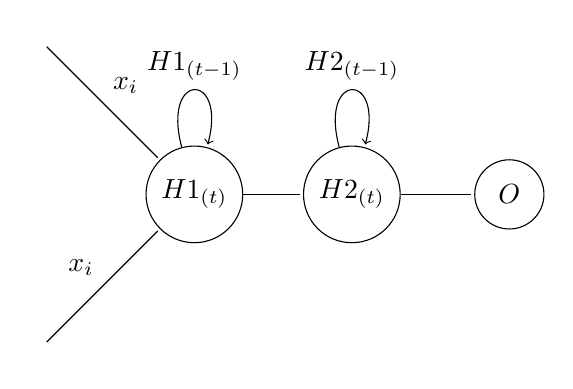
\begin{tikzpicture}[shorten >= 1pt, node distance = 2cm, on grid, auto, square/.style={regular polygon, regular polygon sides = 4}]
	\node[](0){};
	\node[below of = 0](1){};
	\node[below of = 1] (2){};
	
	\node[state, right of = 1](N1){$H1_{(t)}$};
	\node[state, right of = N1](N2){$H2_{(t)}$};
	\node[state, right of = N2](output){$O$};
	
	\draw[-]   (0) edge node{$x_i$}(N1)
	(2) edge node{$x_i$} (N1)
	(N1) edge[loop above] node{$H1_{(t-1)}$} (N1)
	(N2) edge[loop above] node{$H2_{(t-1)}$} (N2)
	(N1) edge (N2)
	(N2) edge (output);	
\end{tikzpicture}
\begin{center}
Iteration number 2 $t=2$
\end{center}
    \caption{A simplified representation of a node in a Recurrent Neural Network}\label{fig:rnn_neuron}
    
\end{figure}
%\clearpage
Figure \ref{fig:rnn_neuron} illustrates the working of a RNN neuron: taking picture \ref{fig:DNN} as a starting point we can see the feedback loop of an RNN node at work.
The first picture shows the state of three nodes in the network on iteration 1: During the feed forward phase the first neuron in the hidden layer one receives input $x$ from the input layer, processes it and passes it on to the consecutive layers; after processing, each hidden neuron saves its working values, and those values form the node's state.  

In the next iteration (shown in the second picture) the process repeats, but this time the  H1 node receives not only input from $x$, but also its previous state as input; it processes the combined values and passes it on to H2, which undergoes the same procedure.

Through this mechanism, the network can better retain knowledge of features from past samples of data, and yield better results.
However this also highlights a potential problem: because each node is only fed its previous state with each successive iteration, as the training process continues the network will develop a bias towards more recent samples of data.
 The cyclical nature of the feed-forward means that at any given iteration the network will retain memory of the initial stages of training, but the influence of those early iterations will wane with time as the network adapts and changes when presented with new data. This phenomenon is usually called 'Gradient Decay'\\
% LSTM might be waaay too much detail. Also fuck its a *masive over-simplificatin*
For some particular tasks such as Natural language generation, gradient decay can significantly influence the final results.

% setup is not enough, since as time goes on the network will develop a bias towards features present in more recent iteration; the influence of data from the older iteration will degrade over time, and the system will slowly tend to 'forget' features and patterns it learned at the beginnning: when it is then presented with new data it has never seen before, thi bias can pose a problem.

%To dampen the effects of this bias one might employ Long-Short Term Memory cells (LSTM), a special kind on RNN neuron which can dynamically rank new information (and by extention, the content of its state) based on its relevance. LSTM ensures that important data is retained regardless on when it was learned, and thus diminishes the effect of the base RNN bias.\newline
%It should be noted however that LSTM does not constitute a straight upgrade from the plain RNN architecture: it may be beneficial in certain cases, but decremental in others.

\subsubsection{Generative Adversarial Networks}\label{subsubsec:gans}
Generative Adversarial Networks are a more complex architecture, composed of two discrete neural networks that are in competition with each other.

The system works by employing a generative network $(G)$ and a discriminator network $(D)$, and figure \ref{fig:gan-diagram} shows its general structure:

\begin{figure}[H]
\centering
    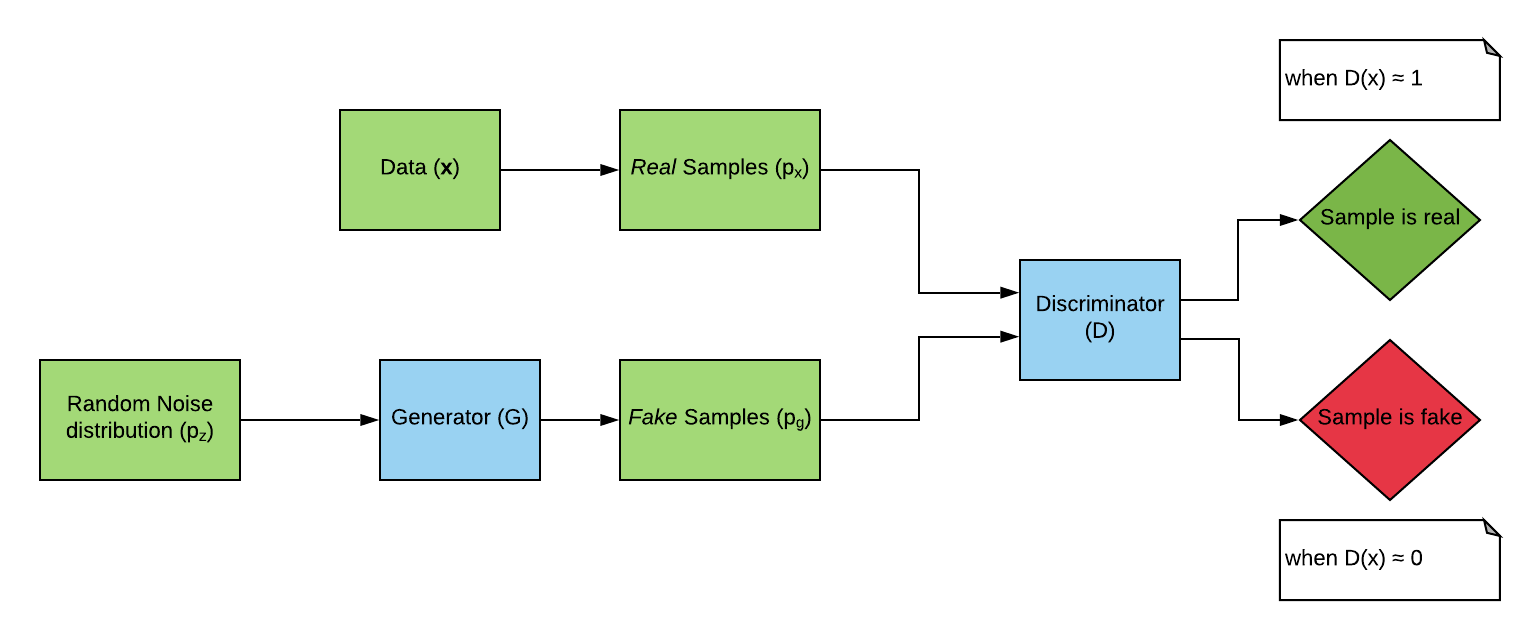
\includegraphics[scale=0.60]{figures/GAN_v2.png}
    \caption{An illustration of the general structure on a Generative Adversarial Network}
    \label{fig:gan-diagram}
\end{figure}    
%Diagram is missing legend

As we can see in figure \ref{fig:gan-diagram}, $G$ generates samples from a random noise distribution $p_z$. We call the resulting data distribution $p_g$; $D$ is fed both data from the training set ($x$) and the output from $G$ ($p_g$), and it's task is to figure out whether any given sample comes from the data (it belongs to $p_x$) or has been generated from $G$ (it belongs to $p_g$). In layman terms, we might say that it is $D$'s job to tell 'real' samples from 'fake' ones.

%The feedback from $D$ is factors into the Error function and helps $G$ improve, and the goal is to train untill $D$ is no longer able to tell the two inputs apart.

%As Goodfellow et al. \cite{Goodfellow2014} explain in their paper, $D$ is trained to maximize the likelihood of assigning the correct label to both data samples and samples from $G$; The generative network in turn is encouraged to generate data that is as similar as possible to the underlying distribution: this creates a race of sorts between the two networks, and a beneficial feedback loop between the two.

Goodfellow et al.\cite{Goodfellow2014} explain the interplay between the two networks as a min-max game: the goal of $D$ is to maximize the likelihood of guessing correctly, while the goal of $G$ is to minimize that same likelihood (or to put it another way, $G$ wants $D$ to make more mistakes): the reason for this is that by minimizing the likelihood of $D$ guessing correctly, we are implicitly telling $G$ to generate samples as close as possible to the input data.

Simply put, the two networks are trying to out-smart each other: every time $D$ tries to spot the 'fake' samples from $p_g$, while $G$ tries to improve more and more to make $D$'s job harder.

The output of $D$ is a single value between 0 and 1 expressing the network's confidence on whether a sample came from $x$; Values of $D(x)$ closer to 1 tend towards assigning a sample to the input data distribution.
Ideally, this race/competition between the two networks comes to an end when the output $D(x)$ stabilizes on $D(x)=0.5$, meaning that $D$ is no longer able to tell the two distributions apart.

%If we trained the network correctly, this will also mean that $p_x=p_g$, and thus we can conclude the training.
This also tells us that if we had infinite resources (both in  data samples and computing resources), we could train until $D(x)=0.5$ and $p_x=p_g$, giving us an output of $G$ that is indistinguishable from the input data.

One important thing to note is that we do not show $G$ any of the input data at any point: all that $G$ has access to is a random noise distribution and the error value for $D$; the Generator has to slowly shape that noise into data resembling the Discriminator's input, by using Gradient Descent.  

The process described above can be formalized in the following general equation:
\begin{equation}
 \min\limits_{G} \max\limits_{D} V(D,G)=\mathbb{E}_{x\sim p_{data}(x)}[\log{D(x)}]+\mathbb{E}_{z\sim p_z(z)}[\log{(1-D(G(z)))}] 
\end{equation} 

Because operation of the network relies on this tight feedback loop between $D$ and $G$, one needs to pay close attention to how quickly each network learn.
The idea, as the authors in \cite{Goodfellow2014} point out, is to have a certain number of iterations of $D$ before we go ahead and adjust the Error for $G$; Conceptually, we might think of this as giving $D$ enough time to tell the real from the fake data reliably (or try), before iterating $G$ to counter $D$'s current strategy.

The original paper indicates this ratio with $k$, and notes that increasing it grows the required computation significantly. In their experiments the authors used a $k$ value of one for performance reasons, while PassGAN defaults to a $k$ value of 10\cite{PassGAN}.

\subsubsection{PassGAN}
% should i mention IWGANs at the beginning? maybe this is a question for Niels.
PassGAN is a generative adversarial network built to generate password candidates for the purposes of password cracking: In it, $G$ and $D$ compete in an attempt to generate passwords that closely mimic the real passwords fed to the network as input data.

In this section, we will go over some of the important hyper-parameters used with PassGAN and some other concepts, that will become relevant is section \ref{sec:testing_and_evaluation} where we put PassGAN to the test.

In order to train PassGAN, we use the passwords from the Libero dataset mentioned in section \ref{subsec:password_cracking}. As is common with deep neural network training, we split our data into two subsets of 80\% and 20\%: the 80\% set that contained the majority of the password would be used for Training, while the 20\% set would be used for Testing. 

 The Training phase is what we covered in section \ref{subsubsec:gans}, but we did not talk about Testing in this chapter: generally speaking testing is the practice of presenting a newly-trained deep learning system with new data it has not seen before, in order to test whether the model performs as expected outside of the limited scope of the training data.

For some simpler machine learning systems like image classifiers (a deep learning system trained to recognized hand-written digits is a very common example), all image data is labelled with what they are supposed to be (\emph{e.g} the label might say what digit a particular image is supposed to be): if we split our data 80\%-20\% like we mentioned before, at the end of training we can present our network with the 20\% of data we put aside and use the labels to quantify whether it can guess as accurately as we expect. As an example of why Testing is needed, one of the risks associated with deep learning systems is \emph{over-fitting}: over-fitting is a phenomenon wherein the network is \enquote{over trained} so to speak, it performs amazingly on the training data but is not flexible enough to maintain that performance with real data outside the narrow scope of training. Intuitively, we might think of it as the network being hyper-focused on the minute characteristics of the training data: it works very well in that specific context but it does not scale well, the features that the network picks up on might not be abstract or general enough to apply in a general case. 

We are discussing the testing process in some depth because there is an important difference between PassGAN and image classifiers: The testing process described above simply does not work with PassGAN.
This is because PassGAN does not simply classify existing data, it creates new and unique data with potentially unseen characteristics: because we do  not know what kind of string PassGAN will generate in advance, we cannot write labels for them; even if we were able to do so, we think that the nature of GANs is at odds with this approach since the interplay between $G$ and $D$ provides the same sort of feedback as labels do on image classifiers.\\
This lack of an easily defined testing methodology or metrics are common among generative deep learning systems, RNNs focused on data generation have a similar issue.

Because of the reasons mentioned above, PassGAN has no built-in method for testing: instead, we have to rely on external methods to test the model's performance.
In this paper we want to test cracking performance, so we use the password candidates produced by PassGAN in rule-based password crackers: this process will be covered in more detail in section \ref{sec:testing_and_evaluation}, for now we will say that we used our 20\% testing password set as the target of our cracking attempts with HashCat and the password candidates coming from PassGAN.\\
To clarify we followed the same testing methodology as Hitaj et  al. \cite{PassGAN}, just using different datasets for training and testing.
\cleardoublepage
Shifting our discussion to the hyper-parameters used with PassGAN, they are values one can change to influence how the training is done. All of the hyper-parameters present in Hitaj et al. \cite{PassGAN} were kept to their default values in this paper. We will briefly touch upon some of them, explain what they do and mention how they influenced our testing of PassGAN.
%IDK if the following part is accurate really.

There are three hyper-parameters that are relevant to this discussion: The first is \emph{sequence length}, a number that defines the maximum length of password candidates generated by PassGAN; this value is set to 10 by default. Sequence length is important because will influence what kind of passwords we use for testing, for the explanation of how sequence length comes into play the reader may look at section \ref{subsec:passgan-testing}.\\
Another important hyper-parameter is the number of total iterations, which defines for how long PassGAN should train: this number is set to $200000$, but PassGAN never reaches the last iteration during our tests: Hitaj. et al. arrived at this value after several experiments as the ideal length of training for their case, however in our paper we have a considerably smaller training dataset of around 530,000 passwords (80\% of the Libero set), so we have noticed that our training stops around iteration number 190000 when PassGAN runs out of input data.

In hindsight we should have tried to tweak the iteration count to optimize for our particular amount of data: we don't really know if this had a negative impact on the resulting model, the extra iterations might have lead to over fitting but we would not be able to tell as we did not have another model trained with a lower number of iterations as a term of comparison.\\
This might be seen as one of the downside of using a generative system like a GAN, testing requires a more elaborate setup and its harder to spot problems when compared to simpler systems with built-in testing methods. 

The third relevant hyper-parameter is $k$, one that we have already discussed at the end of the previous section. As a reminder, $k$ is a value that determines how many iterations of $D$ happen for every iteration of $G$. In effect, it controls how quick the feedback loop between the two systems is and how fast PassGAN learns and adapts. We have not modified $k$ in our testing, but we mention it again here because we think it is key in understanding how PassGAN works. 

\cleardoublepage
\section{Issues with the autenticity of the Libero dataset}
In the next section we will cover our experiments with PassGAN and the Libero dataset.
Before that however we need to address some fundamental issues with the dataset: First, our copy of the Libero database only contained plain texts passwords, and secondly we were unable to verify the exact provenance of this data.
A direct link to the copy of the Libero leak used in this paper can be found on the \texttt{databases.today} website\footnote{\url{https://cdn.databases.today/Libero.it\%20900k.zip}}

As mentioned in section \ref{sec:related_work} the Libero set is a JSON formatted file containing various pieces of information for each of user (around 700,000 user); common fields for each user include email address, user-name and internal User ID, but some users in the document also have a real name attached. As for the passwords, each user object contains both a plain text password and an MD5 hash.
However something is wrong with the hashes: upon closer inspection we find that the MD5 hash is the same for each user, and that MD5 hash encodes the word \enquote{boomerang}.

We have no idea as to why the uploader of the original cracker would choose to do something like that, and no clear evidence towards any particular reason; The following is purely our speculation, but we can imagine for example, that the attacker might decide to throw away the original hash and only keep the pain text of the password in order to keep the information for each user organized and more easily exploitable: since he exfiltrated not just passwords but also personal information like names and addresses for some of the users, one might imagine that it would be convenient to organize all the information for each user in a single JSON object and perhaps leave a placeholder hash in place of the original password hash.

This alteration to what we might normally expected to find - a file containing both plain texts and hashes of those plain text passwords - made us question the authenticity of the data in our possession: while we were unable to find definitive proof, the number of accounts present in our file is roughly consistent with the number reported in \cite{libero_leak}; further more, the hash of the archive matches that of a VirusTotal report, that shows the archive first appeared on VirusTotal in December 2016, a couple of months after news broke about the Libero Mail security breach \cite{virus_total}.
Italian news articles reporting on the incident came out around September 7th 2016, when Libero Mail sent an email to their customers informing them of the breach \cite{libero-news-wired,libero-news-tomhw,libero-news-fanpage}.
Looking at the database file itself, its \emph{mtime} (the time-stamp of when the file was last modified) is dated to September 25th, placing its origin somewhere closer to the date of the incident. Unfortunately neither the news articles nor Libero Mail themselves give an indication of when exactly the incident occurred, so its hard to judge the exact timeline of events; Upon reading the email that Libero Mail sent to customers on September 7th (available in \cite{libero-news-fanpage} in Italian), the language used suggests Libero may have been aware of the breach for a considerable amount of time before breaking the news to customers.

The elements above leads to believe that the data we have is likely to be from the original Libero leak, though ultimately its very hard to know for certain: these accounts and passwords have been re-used and included in a variety of other sources ever since the incident, and if the original leak came from the Tor network like the Virus Total report tags seem to suggest, it might be exceedingly hard to track down the original archive and/or its creator.

The lack of hashed passwords in our copy of the Libero leak did not interfere with training of the PassGAN system, as the input data to PassGAN consisted of pain text passwords, but it did pose a challenge for testing: in order to test PassGAN we needed to crack the Libero leak passwords using HashCat, and thus we needed to turn the pain text passwords back into hashed passwords.
In ordered to do that we hashed the pain text passwords with MD5 and used the resulting file for testing: our choice of MD5 was somewhat arbitrary, as there is no clear indication of how the passwords might have been stored in the Libero Mail database: we chose MD5 because the filename of the database file hinted that that might have been the hashing algorithm used originally, and also because the weakness of MD5 would make the cracking process much faster compared to using SHA-1 or SHA-256; the JSON file contained no explicit indication of salt usage, so we decided to not try to salt the password either. 
However for all the reasons discussed above, its possible that Libero Mail used a more secure storage method with different hashing algorithms and salts, we simply do not have enough information to express a judgement either way.

We are aware that this lack of information and authenticity hurts the applicability of this paper, because of these compromises we cannot claim that our results are 100\% applicable in the real world. Out argument would have been more robust if we had a dataset that more closely matched the original way in which passwords were stored, but we argue that this paper is not focused on the real-world applicability of Machine Learning systems like PassGAN for password cracking. 
Rather, we view the Libero leak as an example, a source of data to evaluate PassGAN when used on non-english passwords and experiment with the impact on Natural Language on password cracking.

\newpage
In order to prepare the data from the Libero leak for both training of PassGAN and subsequent testing we used a combination of UNIX shell commands, displayed below:

\begin{lstlisting}[language=bash,numbers=left,stepnumber=1,breaklines=true,postbreak=\mbox{\textcolor{red}{$\hookrightarrow$}\space}]
#Extract passwords from the databse file
cat libero.it-lebero-poinx21.pxusers-plaintext-md5-2016-09-json-900k-users-extremely-private.txt|grep clearPassword |cut -d ":" -f 2 | awk '{gsub ("\"","");gsub(",","");print $1}' > passwords.txt

#Split the entire password dataset into 80%/20%
head -n 534171 passwords.txt|shuf > train.txt
tail -n 133542 passwords.txt|shuf > test.txt

#Extract passwords that are 10 characters or less (needed for testing)
grep -x '.\{1,10\}' test.txt > test_10c.txt

#Generate MD5 hashes of the testing set for Hascat
for i in $(cat test_10c.txt); do echo -n "$i"| md5sum | tr -d " -" >> test_10c.hash; done

#Generalized parameters for Hashcat
hashcat -a 0 -m 0 --potfile-disable test_10c.hash $WORDLIST -r $RULESET -o out.txt
\end{lstlisting}


\cleardoublepage
\section{Testing and evaluation}\label{sec:testing_and_evaluation}
In this next section, we are going to evaluate the performance of the PassGAN system on the Libero set, as well as give a brief overview of our methodology and the experimental setup.

\subsection{Experimental setup}
Both training of the GAN and testing were carried out on a Linux machine running Debian stretch, equipped with a GTX 1070 graphics card, an i5-2500 CPU and 8 GB of system memory. 
With this card, training of PassGAN took roughly twelve hours.
PassGAN was run on Python 2.7, running Tensorflow 1.12.0.%\\

For testing we used the latest stable version of HashCat available at the time (version 5.1.0). %and we observed a peak speed between 850 and 860MH/s (for reference, 1MH/s is equivalent to 1 million candidate passwords hashed and compared per second) %Reference  %The definition of MH is probably wrong

%change position of NL box and make legen entry for optional things green
Figure \ref{fig:testing_flowchart} below illustrates our overall process, which is divided in two Phases: 
\begin{itemize}
    \item A Training Phase, in which we train PassGAN on a given dataset and sample password candidates from the trained model.
    \item A Testing Phase, in which we use HashCat to try and crack a sub-set of the passwords in the libero leak.
\end{itemize}

\begin{figure}[H]
\centering
    \includegraphics[scale=0.7]{figures/testing_flowchart_ocd.png}
    \caption{A diagram illustrating our general workflow for evaluating PassGAN, including Training and Testing}
    \label{fig:testing_flowchart}
\end{figure}    

\subsection{Training the PassGAN system}\label{subsec:passgan-training}
As we explained back in section \ref{subsubsec:gans-passgan}, in order to train PassGAN we took the plain text passwords from the libero leak (667,714 passwords) and split them into two groups. 80\% of the passwords went into our Training Set, while the remaining 20\% of passwords went in the Testing set: the Training set is used to train PassGAN as can be seen in Step 1 of Figure \ref{fig:testing_flowchart}, while the passwords in the Testing set are hashed with MD5 to serve as a cracking target for HashCat as seen in Step 2 of figure \ref{fig:testing_flowchart}. We will go into further detail with the Testing set in section \ref{subsec:passgan-testing}, as the brief explanation provided here is not entirely accurate.

PassGAN can additionally be trained on Natural Language data, shown in a dotted box in figure \ref{fig:testing_flowchart}; elements shown within a dotted box are considered optional, they can be included or not. Natural Language data will be further discussed in section \ref{subsec:nl-testing}.

Once PassGAN is done training with a given dataset, it produces a trained model that can be used to generate candidate passwords via sampling (Step 1.1 in figure \ref{fig:testing_flowchart}).\\ 
We covered the concept of models back in section \ref{subsubsec:gans-passgan}, but as a reminder a model is a snap-shot of the internal state of a network, containing all the weights and parameters necessary to process new input (or generate password candidates with the features learned from the training data, in the case of PassGAN).

We can use the trained model produced at the end of training to sample password candidates generated from PassGAN: The result of the sampling process will be a list of candidate passwords that make up the PassGAN wordlist used with HashCat when testing. We can choose to generate more or less candidate passwords when sampling: the tests listed in table \ref{tab:test-set} use a wordlist of 1 million password candidates, while tables \ref{tab:passgan-big} and \ref{tab:nl-results} use a wordlist of roughly 14 million password candidates.


%In order to train the PassGAN system, we extracted the plain text passwords from the original file (which was formatted in JSON as it contained personal information beyond just the emails and passwords of the users), and split it up in two sets: a training set containing 80\% of the passwords (534,171 entries) and a testing set containing 20\% of the passwords (133,542 entries).
%We used the model trained on the bigger set to generate 1 million samples from PassGAN, that then served as the basis from our initial testing.

Below is a small sample of password candidates generated by PassGAN, taken from the 1 million wordlist: %Maybe i should take a sample from the last checkpoint instead?
\begin{verbatim}
22052906    mariamuna   iaup63     poldetta53
001178      04051987    topolapa    aenara
rotsanera   princone    fadyreda21  giugki
dimonepa72  12orlomon   deb57828    belnabola
marcanalla  ACADCNAN   leegenniki  vicaletto
\end{verbatim}

%Give a small example of one or two particular words and words in italian that resemble them.
What we found particularly interesting was that while the samples showed the typical patterns exhibited by user-generated passwords (numbers appended or pre-pended to words, so-called leet speak etc..), a majority of them also seemed to mimic Italian words and phrases: most of these words were meaningless, but nonetheless we speculated that the GAN might be trying to \enquote{learn} Italian as a side-effect of generating samples close to the input data distribution.
As an example the string \texttt{vicaletto} resemble the italian word \enquote{vicoletto} meaning \enquote{a narrow street}, while the string \texttt{princone} sounds vaguely like the italian word for pickaxe, \enquote{piccone}. 

\subsection{Testing the PassGAN system}\label{subsec:passgan-testing}

\begin{figure}[H]
\centering
    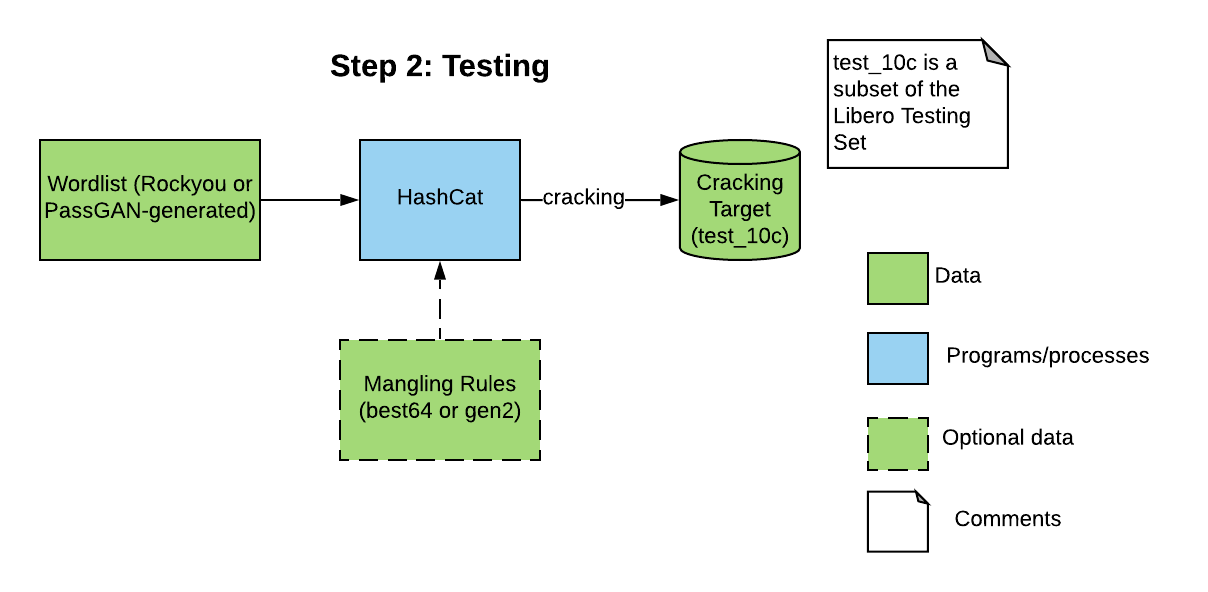
\includegraphics[scale=0.8]{figures/testing_only.png}
    \caption{A zoomed-in version on the previous diagram, showing only the Testing process}
    \label{fig:testing_only}
\end{figure}    

The testing process is depicted in figure \ref{fig:testing_only}: In it we use HashCat to crack a sub-set of the Libero leak passwords (the cracking target), using a wordlist and optionally a set of mangling rules as input.

%This section is still convoluted
The cracking target is a sub-set of the Libero Testing set, that itself is a set of 20\% of the libero leak passwords that we set aside from testing as mentioned in the very beginning of section \ref{subsec:passgan-training}.
% make it more clear that we are copying the passgan paper.
Our cracking target is not the whole Testing set, but a sub-set of it composed of passwords with a length of 10 characters or less: this was done because Hitaj. et al. \cite{PassGAN} also limit their testing with HashCat in this same way, we decided to do it too in order to more closely follow their methodology; as to the reason why this limitation is in place, we speculate this is done to better suit the passwords in the cracking target to PassGAN. As we mentioned back in section \ref{subsubsec:gans-passgan}, PassGAN sets the \emph{Sequence Length} hyper-parameter to 10 during training: this parameter sets the maximum length of password candidates generated by PassGAN during sampling, so testing against a sub-set of 10-character passwords is a way to tailor the cracking target to PassGAn's output slightly.
We do not fully understand why Hitaj. et al. made this choice, but nonetheless we adopted it ourselves in an effort to more closely mimic their evaluation process.

We believe this sub-set of ten character passwords still represents the whole Testing set fairly, as not many passwords were removed: the vast majority of passwords in the Testing set are 10 characters or less, 111,994 or 83.86\% to be precise. 
From here on, we will refer to this sub-set of 10 character passwords as \emph{test\_10c} (the actual filename) or more simply as \enquote{the cracking target}

% During our testing we tried to follow the same sort of methodology that Hitaj et al.\cite{PassGAN} used in their paper: as such our cracking target is not the whole Testing set, a sub-set of it composed of passwords with a length of 10 characters or less: This was done to better use PassGAN, as during training we set the maximum sequence length to 10.
% We believe this sub-set of ten character passwords still represents the whole Testing set fairly, as not many passwords were removed: the vast majority of passwords in the Testing set are 10 characters or less, 111,994 or 83.86\% to be precise. 
% From here on, we will refer to this sub-set of 10 character passwords as \emph{test\_10c} (the actual filename) or more simply as \enquote{the cracking target}

Touching upon the wordlist and rules used, they are also depicted in figure \ref{fig:testing_flowchart}: for the former we use either the \emph{RockYou} wordlist or a wordlist generated by PassGAN, while for the latter we use either the \emph{best64} or \emph{generated2} rule sets. Both the RockYou wordlist and the two rulesets mentioned above were chosen because they were used in Hitaj et al. \cite{PassGAN}, but also because they are widely used and understood to be among the more efficient wordlists available to an attacker. We believe that they demonstrate rather well what rule-based password crackers can do without further language specific optimizations such as those that PassGAN provides. %Reference, nigga

The RockYou wordlist contains more than 14 million passwords, all of which come from various data breaches that have been compiled into one resource; it contains password of varying length and complexity, and as such should provide a good performance baseline for rule-based crackers. The best64 rules file contains around 70 mangling rules, while the genrated2 rules file contains more than 65,000. 

The tables below will illustrate the results of our tests attacking the cracking target with different combination of Wordlists and rules. To clarify, we decided early on to use mangling rules also when testing password samples from PassGAN, since they greatly increased the number of passwords found compared to just using a wordlist. 
To the best of our understanding Hitaj. et al. have not used rules in their evaluation of PassGAN, but instead have chosen to generate a huge number of password candidates and use PassGAN alone to match passwords in the cracking target. We have also briefly tried this approach, our experience with it will be detailed in section \ref{subsubsec:huge-wordlists}}%If you wanna put the results for huge passgan wordlist here is where they go
%This is not something that Hitaji and al. seem to have done, they seem to have used only PassGAN-generated wordlist to crack their target db. We tried and we got really shit results

As a final note, HashCat's default behaviour is to cache passwords found during an attack in what the HashCat manual calls a \emph{potfile}, so that if an attacker chooses to approach the target using a different wordlist or a different set of rules, no time is wasted cracking passwords that were already found previously; because using different rule sets can greatly affect the efficiency of cracking, this form of caching allow an attacker to crack more passwords by combining different approaches.
In order to test the performance of each wordlist and rule combination separately, we disabled caching of cracked passwords between cracking attempts: this was done with the HashCat command showed in the code snippet in section \ref{sec:libero}, and it allowed us to evaluate the performance of different combination of wordlists and rules singularly. However disabling the potfile also leads to a lower overall number of passwords found. Tables \ref{tab:test-set}, and \ref{tab:passgan-big} show show tests done with caching disabled, while the figures obtainable with caching will be mentioned in section \ref{subsubsec:potfile-enable}. 

\begin{table}[H]
\begin{tabular}{|l|c|c|c|}
\hline
\textbf{\emph{Wordlist/Ruleset}} & \textbf{-} & \textbf{Best64} & \textbf{Generated2} \\ \hline
\textbf{Rockyou}          & 19,215 (23.78\%) & 30,170 (37.33\%) & 59,134 (73.18\%) \\ \hline
\textbf{PassGAN}          & 4,637 (5.74\%) & 11,053 (13.68\%) & 34,896 (43.18\%) \\ \hline
\end{tabular}
\caption{A comparison of the number of passwords found in the cracking target by RockYou and PassGAN,  using a 1 million wordlist for PassGAN}
\label{tab:test-set}
\wfill
\hfill
\end{table}

Table \ref{tab:test-set} shows that PassGAN performs rather poorly in comparison with the RockYou wordlist: we attributed this shortcoming to two main factors: firstly the size of the wordlist generated by PassGAN, which is 1 million entries as opposed to the 14+ million entries of RockYou, and secondly the quality of the PassGAN wordlist. Both of these factors play into each other, because while the rules provide great advantages in terms of password found, ultimately they just modify the entries in the wordlist. Thus we might say that the whole system is limited by the capabilities of the wordlist that is used.

In order to test this hypothesis we used our existing PassGAN model to generate a bigger wordlist with as many entries as as RockYou, and performed a second test:
\begin{table}[H]
\centering    
\begin{tabular}{|l|c|c|c|}
\hline
\textbf{\emph{Wordlist/Ruleset}} & \textbf{-} & \textbf{Best64} & \textbf{Generated2} \\ \hline
\textbf{Rockyou}          & 19,215 (23.78\%) & 30,170 (37.33\%) & 59,134 (73.18\%) \\ \hline
\textbf{PassGAN}          &  10,735 (13.28\%) & 20,638 (25.54\%) & 48,751 (60.33\%) \\ \hline
\end{tabular}
\caption{A comparison of the number of passwords in the cracking target found by RockYou and PassGAN, using a 14 million wordlist for PassGAN} 
\label{tab:passgan-big}
\end{table}

As table \ref{tab:passgan-big} shows, PassGAN found roughly 15\% more passwords when using a bigger wordlist: this leads us to believe that wordlist size and quality does constitute a performance bottle-neck. It should be also noted that when compared with the original, 1 million string wordlist, we found a significant 40\% overlap in the strings that were generated. Addressing the problem of quality of the wordlist, we speculated that one of the reasons for the gap in efficiency between PassGAN and RockYou might be the fact that the strings generated by PassGAN don't follow grammatical rules, and this might have hindered the efficacy of the base wordlist. This hypothesis however was later proven wrong by our natural language experiments, detailed in section \ref{subsec:nl-testing}
%Talk about the 50mil and 100mil exapriements

\subsubsection{Running HashCat with caching}\label{subsubsec:potfile-enable}
Now that we had an idea of the performance of each method, we wanted to see what was the maximum number of passwords we could find by combining the two approaches (RockYou and PassGAN):
In order to do this we took the best performing ruleset (generated2), and we performed two rounds of cracking with caching enabled. First we run RockYou with the generated2 ruleset, that yielded the same results shown in Table \ref{tab:passgan-big} for that particular combination; next we tried PassGAN plus generated2, which yielded a final result of 63,847 passwords found (79.01\% of the cracking target). Running the two approaches in combination seems to definitely be more affective that using PassGAN alone, as there are many passwords that PassGAN cannot find but that are cracked by the RockYou wordlist.
Furthermore when we look at the two lists of cracked passwords, we can notice around 5,000 unique passwords that were matched by PassGAN but not Rockyou, showing that PassGAN might have some potential as a tool to close in on more difficult passwords that have a specific linguistic provenance. Looking at some of these unique passwords, they mostly consist of proper names and more obscure italian words.

\subsubsection{Testing the limits of PassGAN wordlist size}\label{subsubsec:huge-wordlists}
As we said previously Hitaj. et al. \cite{PassGAN} don't seem to have used rules when testing PassGAN: instead they seem to have taken a different approach, taking advantage of the fact that PassGAN can generate arbitrary numbers of password candidates from a trained model; these password candidates may not match the target as well as the passwords in an established wordlist like RockYou, but PassGAN can generate vast quantities of them: thus Hitaj. et al chose a \enquote{quantity over quality} approach.

We were interested in seeing how such huge wordlists would perform without the help of rules, so we run a couple of tests: we took our existing PassGAN model, our standard cracking target \texttt{test\_10c}, and we generated three new wordlist for PassGAN: one with 50 million entries, one with 100 million entries And finally one with roughly 196 million entries. 
The reason why we chose these 3 steps is simple: as we can see in tables \ref{tab:test-set} and \ref{tab:passgan-big}, going from 1 million entries to 14 million entries yielded 15\% more passwords, so we wanted to see if testing a wordlist with $14^2$ million passwords would yield roughly 15\% more results compared with table \ref{tab:passgan-big}. The 50 million and 100 million wordlists are intermediate steps that can give us clues on how the number of passwords scales with wordlist size.
%The 50 million wordlist managed to crack 13.898 passwords (17.20\% of the cracking target), while the 100 million wordlist managed to crack 15.669 passwords (19.39\% of the target).\\
%While the increase between the two
\begin{table}[H]
\centering    
\begin{tabular}{|l|c|c|c|}
\hline
\textbf{\emph{Wordlist/Ruleset}} & \textbf{-} & \textbf{Best64} & \textbf{Generated2} \\ \hline
\textbf{PassGAN (50 million passwords)}          & 13.898 (17.20\%) & - & - \\ \hline
\textbf{PassGAN (100 million passwords)}          & 15.669 (19.39\%) & - & - \\ \hline
\textbf{PassGAN (200 million passwords)}          & 17.523 (21.68i\%) & - & - \\ \hline
\end{tabular}
\caption{A comparison of the number of passwords found by just PassGAN using different wordlist sizes and no mangling rules} 
\label{tab:passgan-big}
\end{table}

\subsection{Training PassGAN with Natural Language corpora} \label{subsec:nl-testing}
%Find a more reader-friendly explanation for grammatical correctness, especially at the beginning  when defining the goal.
Our next step was to include natural language data in the input and re-train the model, in the hope that this new input data would help the system generate more grammatically correct strings and thus improve the number of passwords matched.

Firstly though we should define what our goal was for using Natural Language with PassGAN, and what we mean with grammatical correctness. 
As we showed at the end of section \ref{subsec:passgan-training}, a sizeable number of the password candidates generated by PassGAN during sampling are words: in the context of the strings generated by PassGAN, we define a \enquote{word} as simply a string composed of uppercase and/or lowercase letters. It might be entirely composed of letters like the two examples we gave in section \ref{subsec:passgan-training}, or have numbers pre-pended or appended to it. As we mentioned in those examples, most of the words generated by PassGAN when trained on passwords exclusively are meaningless: they may resemble italian words, but they are ultimately incorrect.
%whats wrong with saying grammatical correctness is that peple may think about sentences adn passphrases
Our goal for training PassGAN with natural language data was to hopefully teach the system enough about the italian language to turn a decent part of those meaningless words into actual italian words. In Turn, we thought, that might have yielded better results in terms of number of password cracked and especially in terms of their quality: We hoped the inclusion of Natural Language data would allow us to match more language-specific passwords like those 5,000 unique passwords mentioned in \ref{subsubsec:potfile-enable}   

% the two corpoora were put toghether by other people, i simpl sampled them.
% say that and cite sources
%Maybe put an excract from the 2 corpora in here too.
For this purpose we have chosen two different corpora of Italian Natural Language samples: 
\begin{itemize}
    \item The Repubblica corpus: A corpus of words extracted from the italian newspaper \enquote{Repubblica}, taken from articles published between 1985 and 2000 (roughly 380 million words).\cite{repubblica_corpus}
    \item The ItWaC corpus: A large 2 billion word corpus obtained by crawling internet sites under the \texttt{.it} domain. \cite{itwac_corpus}.  
\end{itemize}

%You can increase the number of guesses by generating more samples and increasing the size of the wordlist, though there might be diminishing returns at some point.
%The nice thing about PassGAN is that you have theoretically infinite wordlists, even if the quality might be up and down.
Both corpora were generated using the NoSketch Engine online tool \cite{nosketch_engine}, and we decided to sample one dataset from each corpus with the same number of entries as the libero password set: we sampled 700,000 words from both the Repubblica corpus and the ItWac corpus, and those two files served as the basis for our Training. This was done to ease the process of organizing data for training PassGAN, and also because we were interested the impact that different ratios of password data to natural language data might have on the resulting model.
Previous research \cite{Melicher2016} has suggested that introducing Natural Language data into a system trained on passwords tends to generate a lot of noise during training, and our results turned out to be in line with that paper.

Both corpora were simply a list of italian words, ranked by their frequency in the corpus: the file produced by the NoSkecth tool has a list of words in descending frequency and their frequency count.
In order to prepare the data for training, went through a similar process to what we did for the libero leak passwords: we divided each corpus into an 80\%-20\% (we realized later this step was entirely unnecessary, as we had no intention of using NL data as a cracking target) and then proceeded to make two wordlist out of each natural language corpus.

The shell commands we used to accomplish this are shown below:

\begin{lstlisting}[language=bash,numbers=left,stepnumber=1,breaklines=true,postbreak=\mbox{\textcolor{red}{$\hookrightarrow$}\space}]
#Split each NL corpus into 80%-20% (not strictly necessary)
head -n 534172 Repubblica_700k.txt|cut -f1 > Repubblica-80.txt
tail -n 133543 Repubblica_700k.txt|cut -f1 > Repubblica-20.txt

head -n 534172 ItWac_700k.txt|cut -f2 > ItWac_80.txt
tail -n 133543 ItWac_700k.txt|cut -f1 > ItWac_20.txt

#Create training data for PassGAN with password data + 50% of the Repubblica corpus
shuf -n 267086 Repubblica-80.txt|cat - ../libero\ it\ July\ 2016/train.txt|shuf > libero+Repubblica-50.txt

#Create training data for PassGAN with password data + 100% of the repubblica corpus
shuf Repubblica-80.txt|cat - ../libero\ it\ July\ 2016/train.txt|shuf > libero+Repubblica.txt

#Create training data for PassGAN with password data + 50% of the ItWaC corpus
shuf -n 267086 ItWac_80.txt|cat - ../libero\ it\ July\ 2016/train.txt|shuf > libero+ItWac-50.txt

#Create training data for PassGAN with password data + 100% of the ItwaC corpus
shuf ItWac_80.txt|cat - ../libero\ it\ July\ 2016/train.txt|shuf > libero+ItWac.txt
\end{lstlisting}

As we can see in the code snippet above, we created two training datasets for each corpus: one contained all the passwords in the Libero Training set and 50\% of the Natural language data, while the other contained all of the Training set passwords and all of the Natural Language data: we did this because we wanted to see what impact different amounts of natural language data had on PassGAN's performance (if any).

We thus proceeded to train 4 separate instances of PassGAN with our four datasets, and then sampled each trained model for testing: the results were 4 separate wordlists, each of around 14 million entries, that we used in HasCat to attack the same cracking target that we used in the previous section (test\_10c).

Touching upon the impact of NL data on the model performance, our hypothesis was that we might see a decrease in model performance when training with 100\% of the natural language data since each corpus contains as much data as the Libero Training set; By combining the two into a single dataset for training, we effectively use as much NL data as password data.  We though this might lead to noise and ‘confuse’ PassGAN, resulting in a model with less focus on generating passwords and more focused on generating NL samples. While that is technically true, overall table \ref{tab:nl-results} shows that the introduction of NL data does not seem to have any noteworthy impact on cracking performance.

The results of our tests on all four wordlists are shown in table \ref{tab:nl-results} below.

\begin{table}[H]
\centering
\begin{tabular}{|l|c|c|c|}
\hline
 \textbf{\emph{Wordlist/Ruleset}} & \textbf{-} & \textbf{Best64} & \textbf{Gen2} \\ \hline
 \textbf{Libero+Repubblica 50\%} & - & - & 51,232 (63.40\%) \\ \hline
 \textbf{Libero+Repubblica 100\%} & - & - &  48,651 (60.20\%) \\ \hline
 \textbf{Libero+ItwaC 50\%} & - & - &  50,133 (62.04\%) \\ \hline
 \textbf{Libero+ItWaC 100\%} & - & - &  47,646 (58.96\%) \\ \hline
\end{tabular}
\caption{Number of passwords found using PassGAN, trained on passwords and Natural Language data}
\label{tab:nl-results}
\end{table}

As we can see the results of training with natural language data are very similar to just using PassGAN+gen2 as shown in table \ref{tab:passgan-big}; there is a slight improvement of 2-3\% when using the datasets containing 50\% of language data, but we do not believe it is a significant change. This result seems to be in line with Melicher et al.\cite{Melicher2016}, and it seems to show us that natural language data does not have much of an impact on the output of PassGAN. 
%\newpage
If we take a random sample from the Repubblica 50\% set, the one that performed the best even if marginally so, we can see that there has not been a substantial improvement in the grammatical correctness of the words in the sample.:
\begin{verbatim}
c3b243dc    fetemanio   carcilla    RATS1203
valentto    itefis82    carmoinx    gip1904
sederonco   elestarsia  220689      QunkYYTx84
n!utelo     kedea       Colpudari   rich1770
aletsa      simoshero   gidni12     1uva1[78
\end{verbatim}    

The words that PassGAN generates are still meaningless and do not seem to have a higher degree of grammatical correctness, the only change we have been able to observe is in the fact that more strings seem to be composed of letters exclusively.

This does not discredit the use of Natural language as a whole, but points us toward the fact that natural language generation and password generation might two different workloads that may not be accomplished well with the same machine learning system: it seems that introducing Natural Language data into PassGAN simply adds noise to the system and does not contribute to the system's performance.
The results in table \ref{tab:nl-results} and the effectiveness of mangling rules as a cracking tool also hint at the idea that user-generated passwords may be defined by their patterns more than by their language of origin.

\cleardoublepage
\section{Discussion}\label{sec:discussion}

In this coming section we are going to discuss some of the shortcomings of this thesis and talk about avenues for future work.

While we were overall pretty happy with the results we obtained from our testing, we feel that there are some deep-seated problems in our arguments that we need to address:

First, its the fact that we did not try to crack the Libero passwords using the pre-trained PassGAN model that Hitaji et al. \cite{PassGAN} used in their paper: we think this is a rather important omission, as doing that would have given us a base-line performance that we could compare our PassGAN model to.  This comparison would have allowed us to determine what were the effects of using a model trained on largely english-language passwords to crack a dataset of italian passwords. We feel such an experiment would have given us much better footing when we claim to be evaluating PassGAN using italian passwords and answering the questions in our problem formulation. As it stands we are still evaluating PassGAN in that way, but not having the reference point of that performance comparison makes our evaluation less meaningful.
This omission is due mostly to time constrains, but also because during our testing process we were wholly focused on the impact of natural language on PassGAN's performance: we really did believe that it would improve performance, and we overlooked some other important experiments such as the one described above that would strengthen our arguments in pursuit of the natural language experiments. 

%Since the beginning the goal of this paper was to test the impact of natural language on PassGAN, and because we were so focused on that objective we skipped over the important experiment outlined above; 
%speaking more broadly we gradually convinced ourselves that natural language would have a positive impact on the model's performance, and in a way we shaped the paper expecting to arrive at that conclusion:
%when we got back the results and realised that the numbers disproved our hypothesis, we gradually realized that our contributions were not as solid as we had hoped.
Speaking of avenues of further work, there were some aspects of our thesis that we would have liked to expand upon:
When discussing the impact of Natural Language data on PassGAN we mentioned that different ratios of password data to Natural Language data affect the model performance in different ways: while we observed 
that PassGAN performs marginally worse when using equal parts of password data and NL data, it would have been interesting to explore this further: we would have been interested in researching what is the ideal ratio to maximize PassGAN performance. \\
A similar argument might be had concerning wordlist size for PassGAN: In section \ref{sec:testing_and_evaluation} we briefly touched upon using even bigger PassGAN wordlists; We believe it would be natural to wonder whether there are diminishing returns concerning wordlist sizes, i.e if there is a point at which adding more words does not lead to a meaningful increase in the number of password size.
In our experience it takes a huge number of password candidates sampled from PassGAN in order to crack passwords without the use of rules, and there might be a point at which PassGAN might stop producing 
unique password patterns leading to a slump in the number of password found. One of the advantages of machine learning systems such as PassGAN is that they can keep producing new password candidates almost 
indefinitely, so we feel that such research might be beneficial in understanding the limits of these systems and also their applicability. Regardless of this potential, as we showed in section 
\ref{sec:testing_and_evaluation} PassGAN can still be useful as a specialist tool to target complex passwords when used in conjunction with rule-based password crackers.

Looking back at our work in this paper, we also realise that it might have been a good idea to attempt to reproduce the findings in the PassGAN paper: it would have helped us to better ground our discussion 
in the context of their paper, but overall we do not think such attempts at reproduction are strictly necessary: while we have certainly looked at Hitaji et al.'s data to give us a broad indication of performance, we were using a different dataset and we don't believe that it would have been meaningful to directly compare our results with theirs.

Our favourite way to build on this paper would no doubt be to do a follow-up study looking at passphrases, as a way to test the limits of PassGAN as a language-sensitive specialist cracker: one might make the case that by their nature, passphrases are more subject to grammatical and syntactical rules, and it would be interesting to repeat the experiments in this thesis using passphrases as a dataset. \\
As \cite{Melicher2016} states, rule-based password crackers tend to have a ceiling on the length and complexity of passwords they can efficiently crack: A similar study using passphrases might also test the limits of rule-based tools in such a way, that we might find PassGAN to be a more effective tool for this particular niche. The big problem we see with this research is the lack of data: passphrases are not usually widely employed by companies in their password policies, and there is a lower chance of leaked passphrases datasets being available to the public.  

\cleardoublepage
% \section{Experimental notes}
When training PassGAN on the libero set, the samples generates seem to have the genral pattern of user passwords; the network tries to generate strings that look like italian words, but are not. Testing of the output has not been performed yet, but i do wonder if including natural language dictionarie can help the network generate grammatically correct words and phrases.

It is yet to be established how grammatically correct words may affet the cracking.

In the next test i will try and add NL dictionaries and see how it goes. 

My hope is that the network can retain the currect password characteristics, but imporve its ability to generate natural langage fragments. Perhaps trnaference learning might come in handy for this?

\subsection{Update(28-2-2019)}

After a second attempt i finished training the model (runtime was around 11.5 hours). i have a working model i can generate samples with, the same proprieties descrribed above hold after a full cycle of training. It is worth noting that after initially being stuck around \-0.8, the error eventually stabilized around \-0.6; This is the lowest i have seen so far.

I am now ready to test this first sample, probably in HashCat. The plan is to extract the MD5 hashes and run a couple of tests:

\begin{itemize}
\item Run a rule-based attack using RockYou as a control group.
\item Run a dictionary attack using the results of PAsGAN obtained from RockYou (and or Linked in, if i can spare 12 more hours to train)
\item Run a dictionary attack using the results of PassGAN training on the Libero leak.
\end{itemize}

The main goal is to compare the last 2 with each otheer and see what differnces (if any) there are.

After that i would like to train again on the Libero set using NL Dictionaries in the training data (which i have yet to acquire), to see if there is an imporvement or regression in the precentage of password cracked.

\subsection{Update (2-4-2019)}

So after the whole hash debackle i decided to take up Niels' advice (at least for now). I generated MD5 Hashes for the passwords and cracked them in hashcat. I generated MD5 Hashes for the passwords and cracked them in hashcat.

Running hashcat with the rockyou wordlist + best64 rules yielde 140.478 passwords (33.57\%)

Running hascat with only the rockyou wordlist gave me the same exact number of passwords, which is kinda suspicious.

Running hashcat with the italian password outputted from PassGAN gave me 146.352 passwords, a whole 1.4\% more!

Running hashcat on a subset of the linkedIn passwords using rockyou+best64 yielded 20\% of passwords, which makes no fukin sense.


% \cleardoublepage
\thispagestyle{empty}
\printbibliography    
\end{document}
